\section{Overview of neutron \el\ experiments}
In neutron elastic scattering measurements, the same time-of-flight techniques are used:
given a ``starting gun'' when neutrons are produced and the neutron arrival time
at a time-of-flight detector, the neutron energy can be calculated.
However, in contrast to total cross section measurements, neutron elastic scattering
measurements require a monoenergetic neutron beam so that elastically-scattered
neutrons can be isolated. Unlike transmission measurements (e.g., total cross
sections), which measure the neutron scattering integrated
over all solid angles, neutron \el\ cross sections are measured differentially with respect to 
solid angle. To measure the angular dependence, one or more time-of-flight detectors
are moved around the scattering sample on a large goniometer. As the differential cross section 
drops precipitously at large scattering angles, more beam time must be spent at
large angles to generate sufficient statistics.

In transmission measurements, the time-of-flight detector is typically placed
very far from the scattering sample so that it subtends an extremely small solid
angle so that only unscattered particles are detected.
For example, in the neutron \tot\ experimental setup described in Chapter
\ref{TCSExperiment}, the scintillator of the time-of-flight detector subtended
4.5$\times$10$^{-6}$ steradians from the point of view of the samples. Thus, the
contribution to background from isotropic $\gamma$-ray production in the samples is negligible.
In differential measurements,
background from $\gamma$-ray production in the samples may exceed the signal
from elastically-scattered neutrons, especially at backward angles where the elastic
cross section is lowest. Pulse-shape discrimination (\gls{PSD})
techniques must be used to filter out 
$\gamma$ rays, leaving only events from elastically-scattered neutrons.

\subsection{Pulse-Shape Discrimination (PSD)}
To identify neutron- and $\gamma$-ray-induced detector events, pulse-shape discrimination
relies on the different energy-deposition modes of neutrons and $\gamma$ rays.
The scintillator used should exhibit both prompt fluorescence with a
lifetime of a few \nano\second\ (from a singlet
state) and delayed phosphorescence with much longer lifetime in the
\micro\second\ range or longer (from a triplet state). Figure \ref{JablonskiExample} shows the
relevant level structure for molecules of such a scintillator. During a scattering experiment,
incident neutrons deposit energy by collision with scintillator nuclei.
These recoiling nuclei (mostly protons) decelerate rapidly in the scintillating
medium via Coulombic interactions with all electrons in the vicinity,
exciting many scintillator molecules in the
ion track. In contrast, incident $\gamma$ rays interact primarily with
single atomic electrons, which, during their recoil, produce a lower excitation energy density.
For the same total energy deposition,
neutron-initiated events produce a higher 
concentration of excited scintillator molecules than do $\gamma$-ray-initiated
events.

In each population of excited scintillator molecules, most molecules are in a
singlet excited state, and they decay promptly by fluorescence back to the
ground state. A small fraction remain in a triplet excited state,
either due to their initial excitation to a
triplet state or because of intersystem crossing from a singlet state. Kept isolated, these
triplet-state molecules have lifetimes that are orders of magnitude longer
(\micro\second\ to \milli\second) than the those in a singlet state because of the required spin
flip to return to the ground-state manifold. If, however, two nearby triplet-state
molecules collide and exchange a unit of spin, they can convert to two singlet-state
molecules, one in the ground-state manifold and one in an excited-state manifold. The excited
singlet-state molecule will decay promptly (\nano\second), freed of quantum-mechanical forbiddenness.
Thus, after the initial prompt fluorescence, delayed light output will appear tens
of \nano\second\ later from these triplet-triplet fusion events. The amount of light will be
dependent on the rate of triplet-triplet collision, a second-order kinetics
process associated with the diffusion of excited scintillator molecules in the
medium. For neutron-initiated events, where the concentration of excited molecules is
higher, the delayed light output is correspondingly higher than for $\gamma$-ray-initiated
events. By comparing the tail of the light output signal to the prompt
fluorescence peak, neutrons and $\gamma$-rays can be distinguished. Typically, the differences in
light output are quantified by comparing the integrated charge of the prompt fluorescence peak
with the integrated charge of a section of the delayed fluoresence. Machine learning 
techniques have also been applied to light output data to further improve discrimination 
\cite{Doucet2018} beyond the simple charge-gate-ratio method. Recently, pulse-shape
discrimination has been shown to be possible in certain solid organic crystals (e.g.,
para-terphenyl, which is also used in laser dyes).

\begin{figure}[tb]
    \centering
    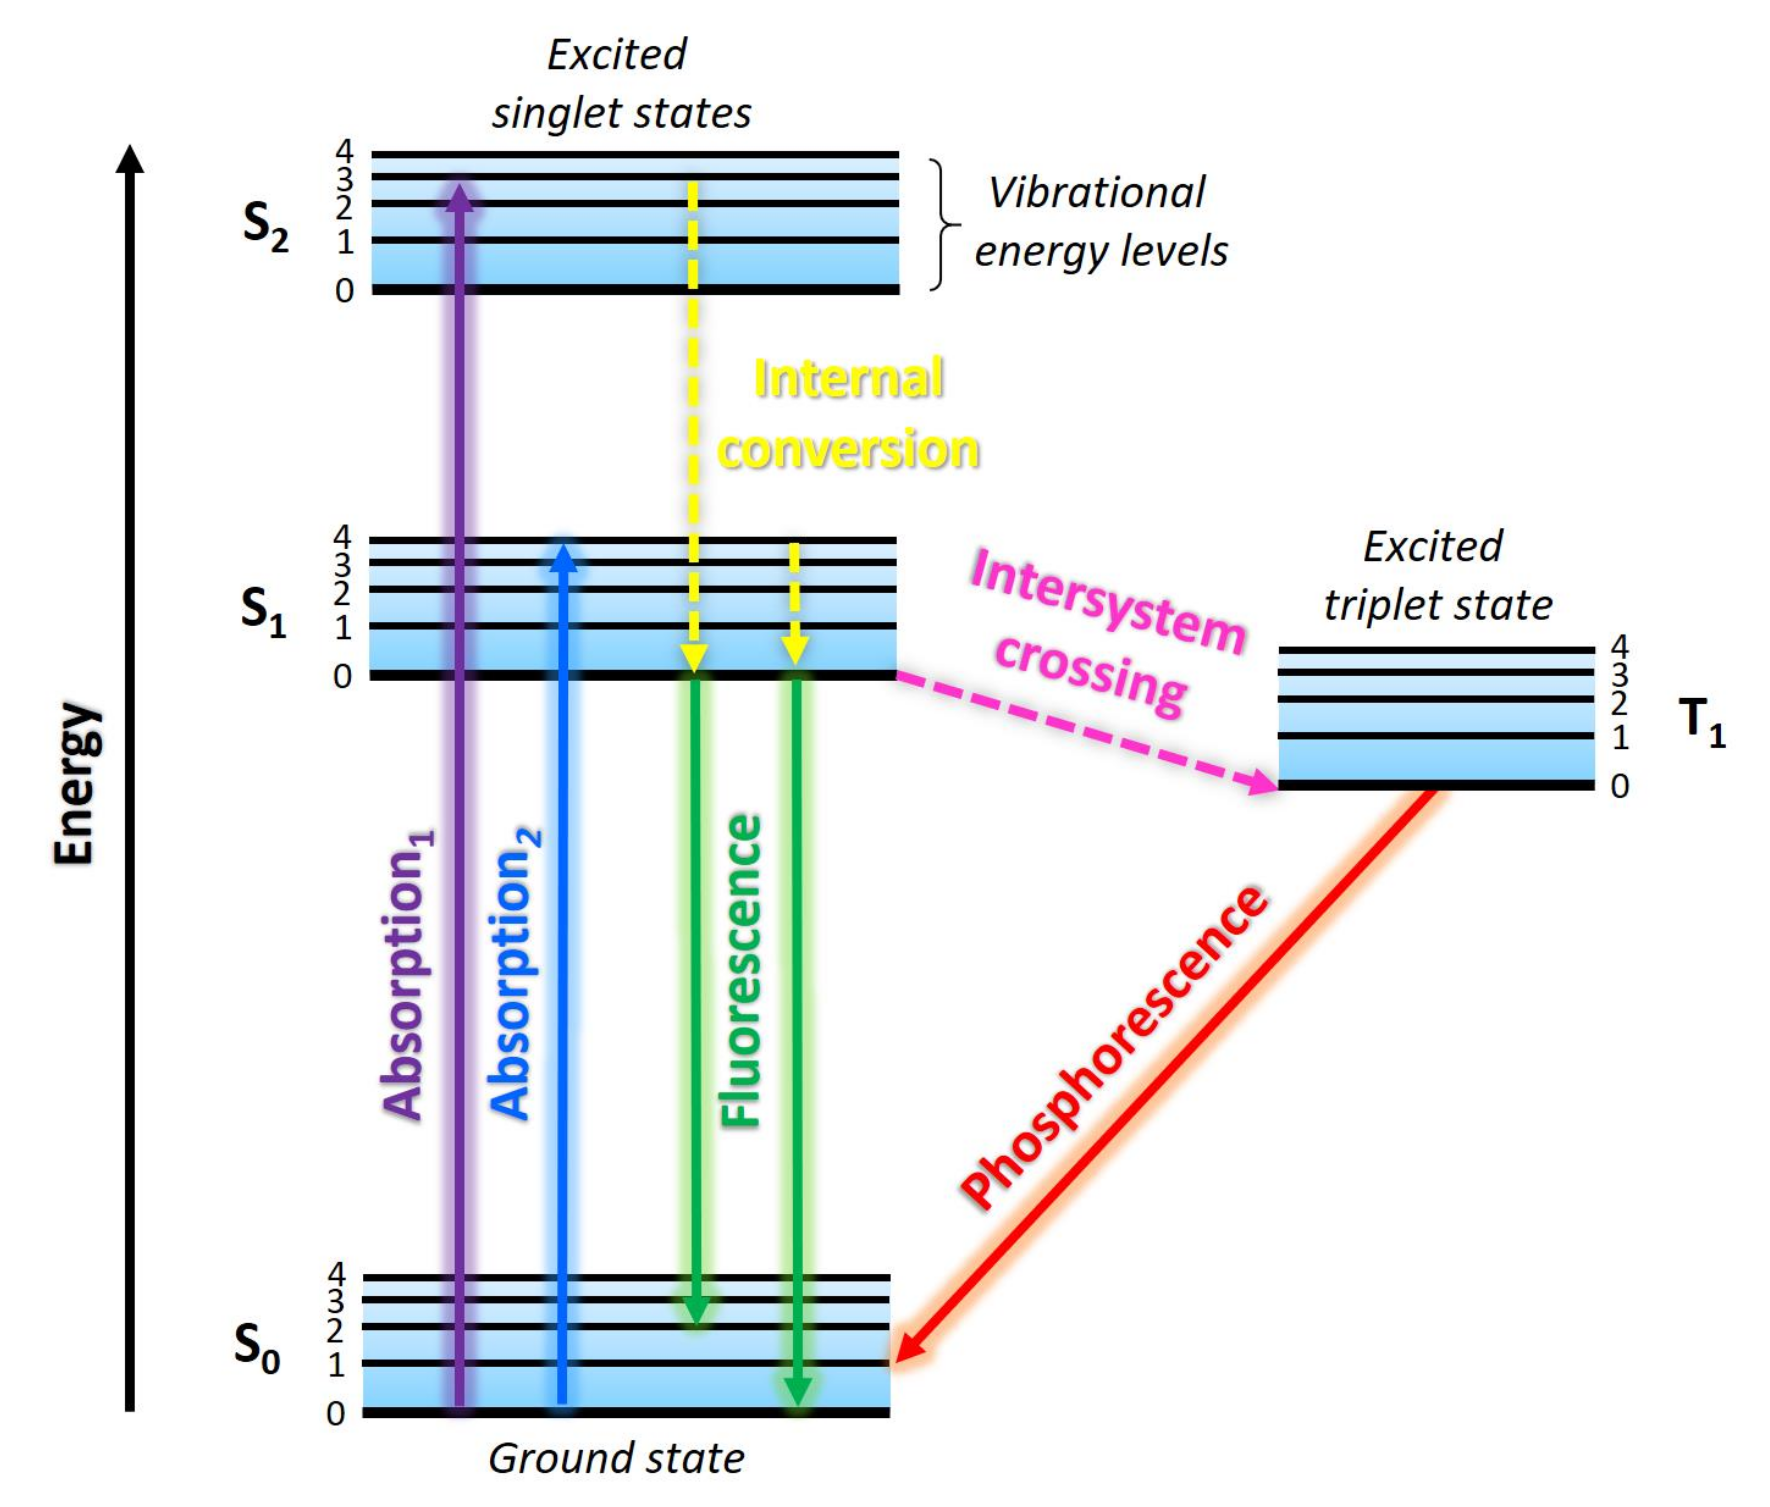
\includegraphics[width = 0.9\textwidth]{figures/JablonskiExample_KangDissertation.png}
    \caption[Example Jablonski diagram for organic scintillator]
    {
        Example Jablonski diagram for an organic scintillator used for
        pulse-shape discrimination. After initial excitation to a higher
        electronic manifold, energy is shed non-radiatively by internal
        conversion on the picosecond timescale. If the first vibrational state of the S1
        manifold is reached, rapid decay to the S0 manifold occurs on the
        \nano\second\ timescale. Alternatively, the system may undergo intersystem
        crossing to the T1 manifold, where it reaches the lowest vibrational
        state. The T1-S0 transition is quantum-mechanically-forbidden,
        dramatically increasing the lifetime of the T1 state and leading to
        delayed light output, or phosphorescence. Figure used with permission 
        from J. Kang \cite{KangPhDThesis}. 
    }
    \label{JablonskiExample}
\end{figure}

In our \snTwelveFour\ neutron \el\ cross section measurements presented below,
we used both \gls{PSD} information and the pulse height of each event to
differentiate neutrons
from $\gamma$-rays (see Figure \ref{PHPSDPlot} in Chapter
\ref{ECSAnalysis}). Our approach follows similar neutron \el\ measurements
conducted at the Triangle University Nuclear Laboratory (\gls{TUNL}) over the last three decades,
including a measurement on \snTwenty\ at 17 \mega\electronvolt\ conducted by Guss et al.
\cite{Guss1989, GussPhDThesis} to which we later compare our results on
\snTwelveFour.

\section{Sample Preparation}
The same \snTwelveNatFour\ samples used in the neutron \tot\ experiment (see Chapter
\ref{TCSExperiment}) were used for our neutron
\el\ measurements without modification. Two additional samples, one of graphite and one
polyethylene, were provided by the TUNL facility in order to normalize our \el\
results using the extremely-well-known (n,p) elastic cross section. The
details of this normalization are given in Chapter \ref{ECSAnalysis}.
The physical characteristics of all the samples are given in Table \ref{ECSSampleTable}.

\begin{table}[ht]
    \caption[Physical characteristics of samples used for neutron \el\
    measurements]
    {
        Physical characteristics of samples used for the neutron \el\
        measurements. For isotopically-enriched samples, the natural abundance
        of the enriched isotope and the isotopic fraction of the sample are
        given.
    }
    \label{ECSSampleTable}
    \begin{center}
        \begin{tabular}{ c c c c c c c }
            \hline
            Isotope & Length & Diameter
            & Mass & Nat. Abund. & Sample Purity\\
                 & [mm] & [mm] & [g] & [\%] & [\%]\\
            \hline

            $^{\text{nat}}$C & 23.58 & 9.39 & 2.924 & - & -\\
            (CH$_{2}$)$_{n}$ & 22.70 & 14.18 & 3.389 & - & -\\

            $^{112}$Sn & 13.65(3) & 8.245(5) &
            4.9720 & 0.97 & 99.9\\
            $^{\text{nat}}$Sn & 13.68(3) & 8.245(5) &
            5.3263 & - & -\\
            $^{124}$Sn & 13.73(3) & 8.245(5) &
            5.5492 & 5.79 & 99.9\\

            \hline
        \end{tabular}
    \end{center}
\end{table}

\section{Experimental Facility at TUNL}
We conducted our neutron \el\ measurements at the neutron TOF
beamline at TUNL (diagrammed in Fig. \ref{ExperimentalSetupTUNL}) in 2017 and 2018.
Incident deuterons, supplied by the
facility's variable-energy tandem Van de Graaff accelerator, impinged on a deuterium
gas cell to produce a forward-focused neutron beam via the d(d,n)$^{3}$He
reaction. This exothermic reaction has a Q-value of 3.269 \mega\electronvolt.
Two measurements, one for 11 \mega\electronvolt\
neutrons and one for 17 \mega\electronvolt\ neutrons, were
conducted. The gas cell pressure varied between 35-40 psi during our
measurement. Per \cite{GussPhDThesis}, we estimate a neutron beam energy spread
at the sample position of 350 keV, mostly from deuterium beam straggling
in the gas cell prior to reacting. The deuterium gas cell
was backed with a fresh tantalum beam stop to prevent unreacted deuterons from
reaching the samples. Based on the number of counts collected during the
normalization runs described below, we estimated that the average neutron flux incident
on the sample was $\approx5\times10^{6}$ neutrons per second for the 11 MeV run
in 2017 and $\approx1\times10^{7}$ neutrons per second for the 17 MeV run in
2018. Of course, the instantaneous neutron flux is much higher due to the pulse
structure of the beam.

The production samples (\snTwelve, \snFour, and a blank) were suspended several
\centi\meter\ downstream of the gas cell in a vertically-aligned wire basket apparatus.
In addition to the production runs, a few normalization runs were taken
with the TUNL-supplied samples (graphite, polyethylene, and a blank).
Between runs, samples were rotated into position
with a hand-actuated pulley. Sample alignment with the gas cell was confirmed
by transit. Neutrons scattering off the samples were recorded by one
of the two main time-of-flight
detectors, designated ``4M'' and ``6M'', roughly 4 and 6 meters away from the target.
These detectors were mounted on large, movable carriages, or ``arms'',
that could be rotated to different angles independently so that two angular
measurements could be conducted simultaneously. By recessing the detectors deep within
the arms' heavy shielding, only neutrons entering the arm at a precise angle
were counted. The active volumes of the 4M and 6M detectors were composed of
NE218 organic liquid scintillator capable of PSD.

To further reduce room background and to shield detectors from direct,
unscattered neutrons,
an ensemble of ``shadow bars'' (wedge-shaped tungsten bricks)
were arranged near the entrance to the detector arms. After an arm's
angle was changed, the shadow bars were aligned by hand so that the
detector had no line-of-sight to the gas cell or the
shielding of the other arm. Any configuration in which the arms were in opposition (i.e., the
angle between the arms was 180$\pm$20 degrees) could allow neutrons scattered
from one arm to enter the detector of the other arm, so these configurations were avoided.

Besides the time-of-flight detectors installed in the arms, a ceiling monitor
detector (CMON) and zero-degree detector aligned with the beam (ZDEG) were used
to record beam flux. In addition, a capacitive pickoff signal
from the accelerator was collected to serve as a time-of-flight
(TOF) stop signal any time an event was recorded on one of the four neutron
detectors. Prior to production, detectors were gain-matched and calibrated with $^{137}$Cs
and $^{22}$Na sources using the Compton edges produced from these $\gamma$-ray sources. For the
4M (6M) detector, a time resolution of 2 ns (3 ns) was achieved for
elastically-scattered neutrons.
An exhaustive description of the TUNL TOF room geometry, detector characteristics,
gas cell, and other apparatus considerations is provided in \cite{GussPhDThesis}.
\begin{figure}[tb]
    \centering
    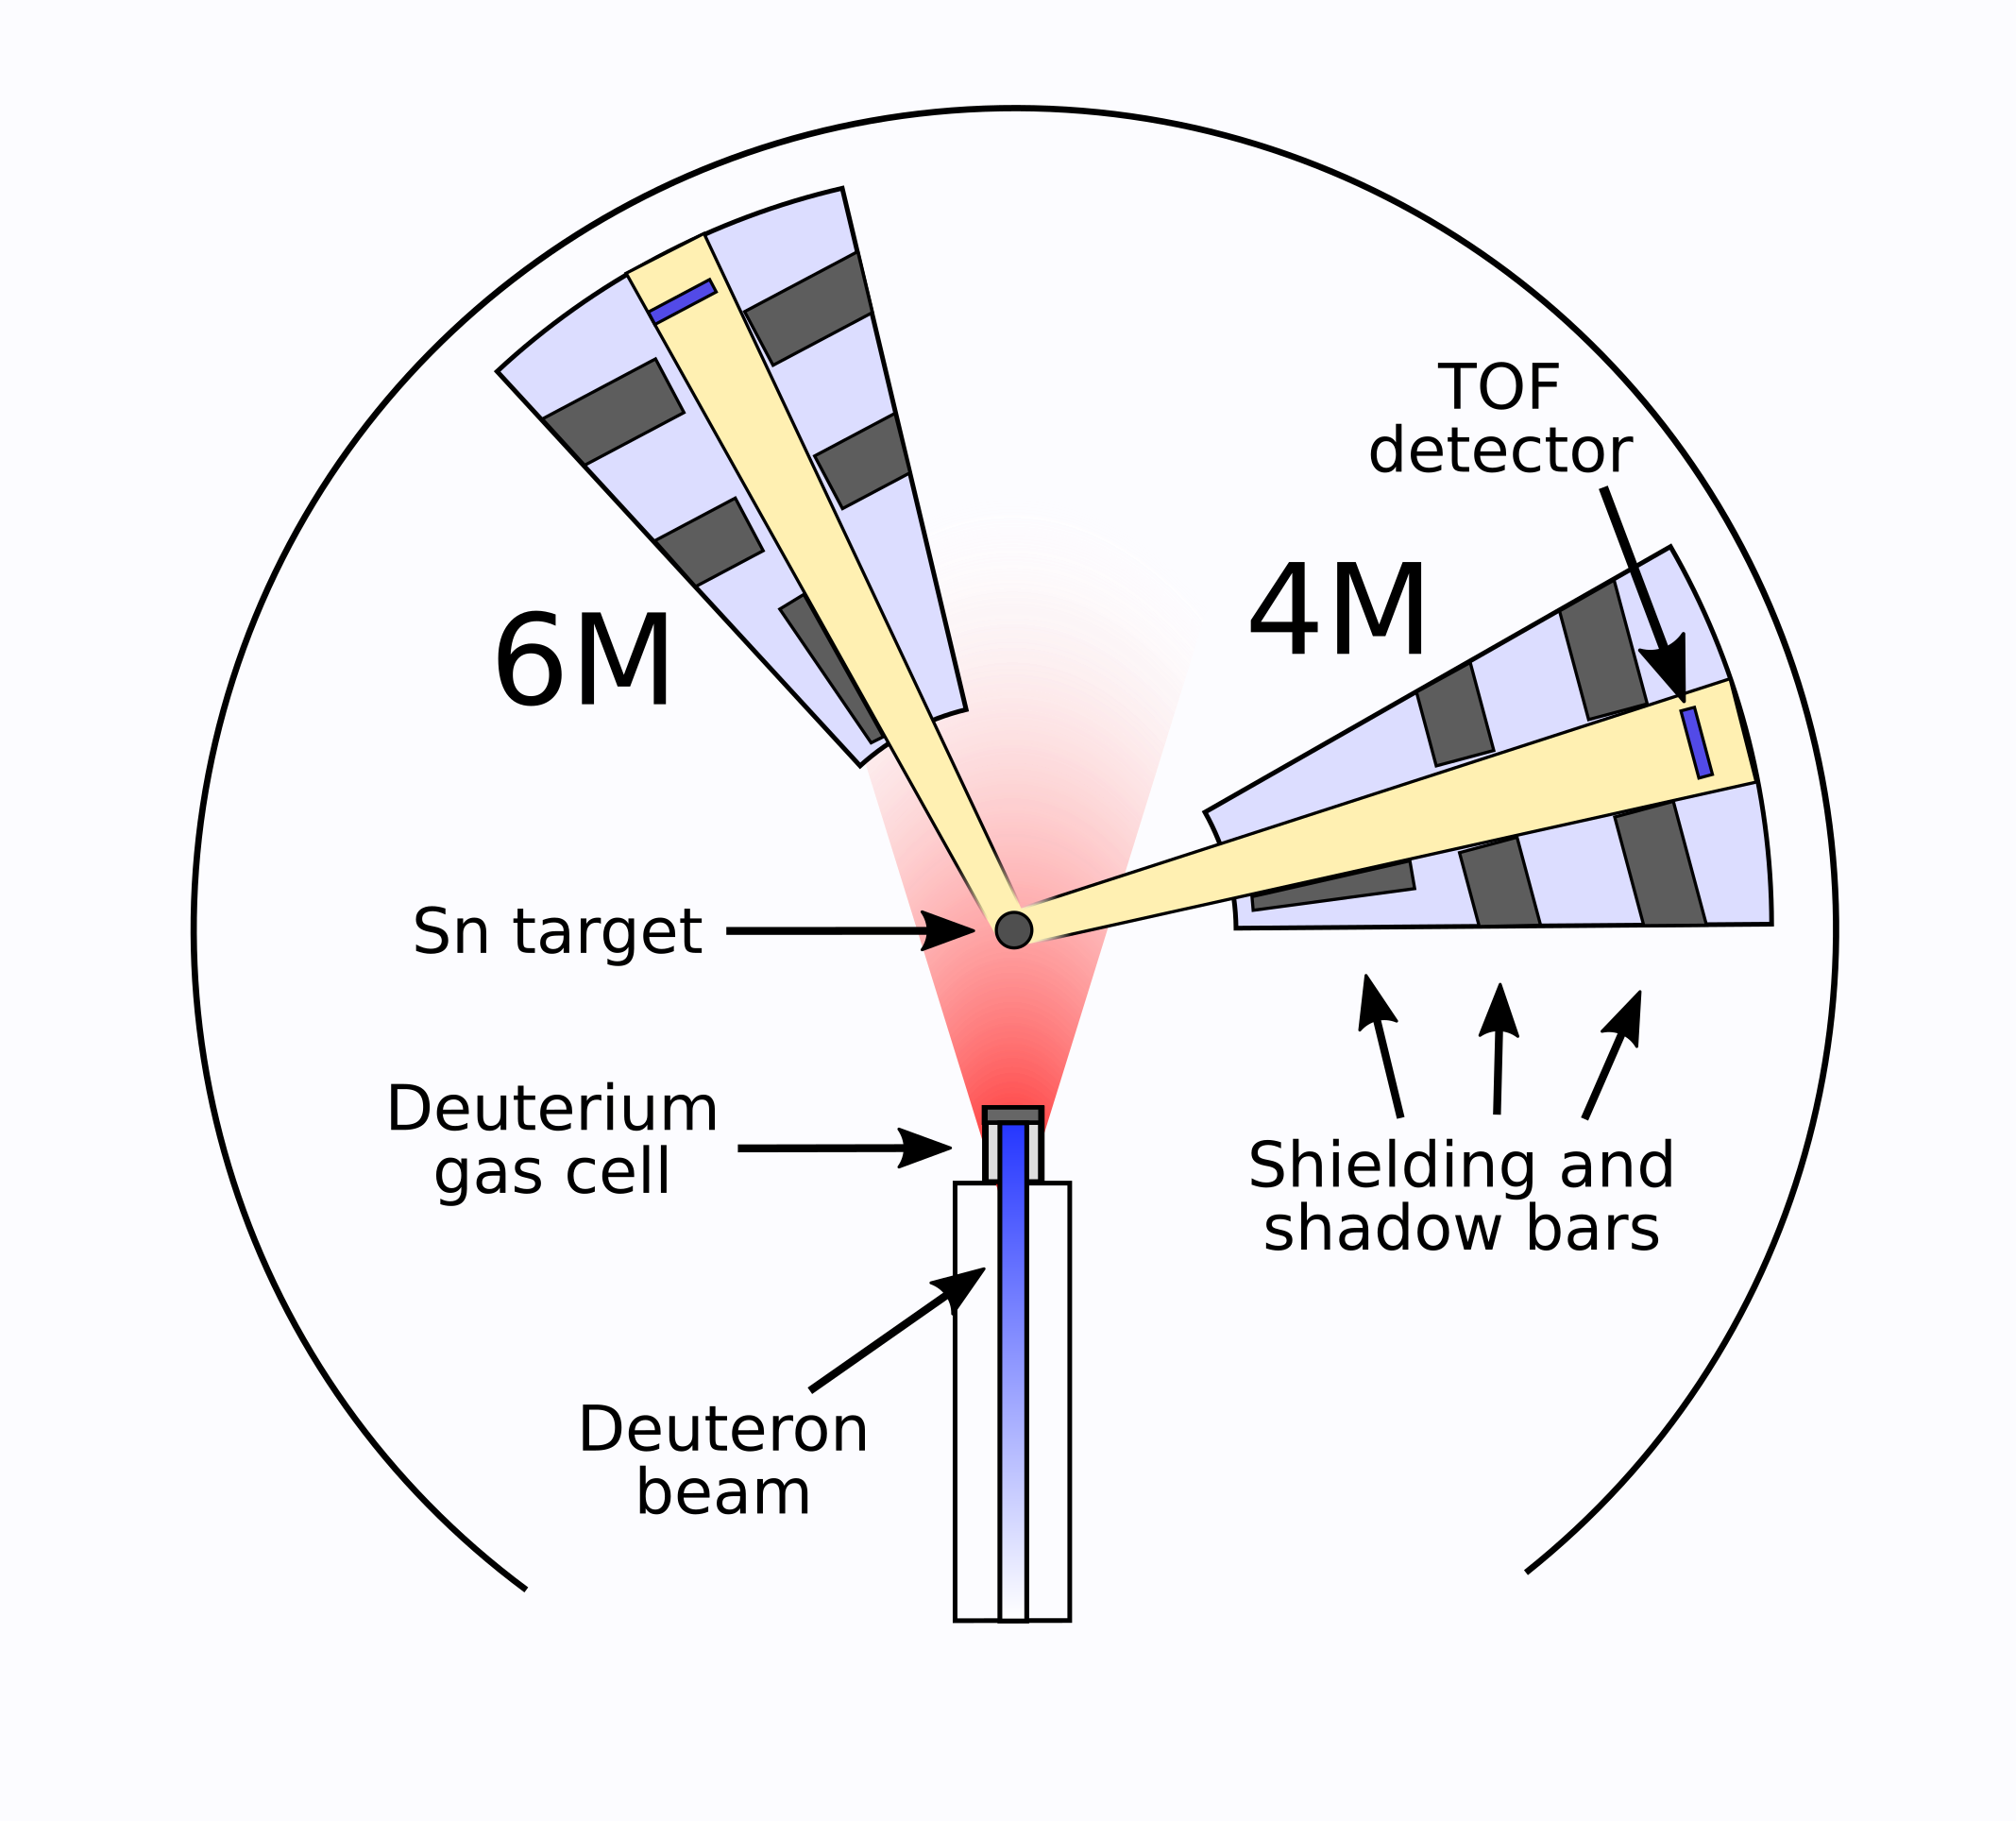
\includegraphics[width = 0.9\textwidth]{figures/ExperimentalSetupTUNL.png}
    \caption[Diagram of the neutron TOF room at TUNL] 
    {
        Diagram of the neutron TOF room at TUNL. Neutrons are produced by d(d,n)$^{3}$He reaction in
        a small gas cell, forming a forward-focused cone (in red). They scatter
        off the sample into one of the detector arms, labeled 4M and 6M, where the neutron
        times-of-flight are recorded. Another shielded detector (not pictured), suspended from the 
        ceiling, serves as a flux monitor so that absolute cross sections can be
        recovered. The angle of each detector arm is read from a goniometer in
        the center of the room.
    }
    \label{ExperimentalSetupTUNL}
\end{figure}

\begin{figure}[tb]
    \centering
    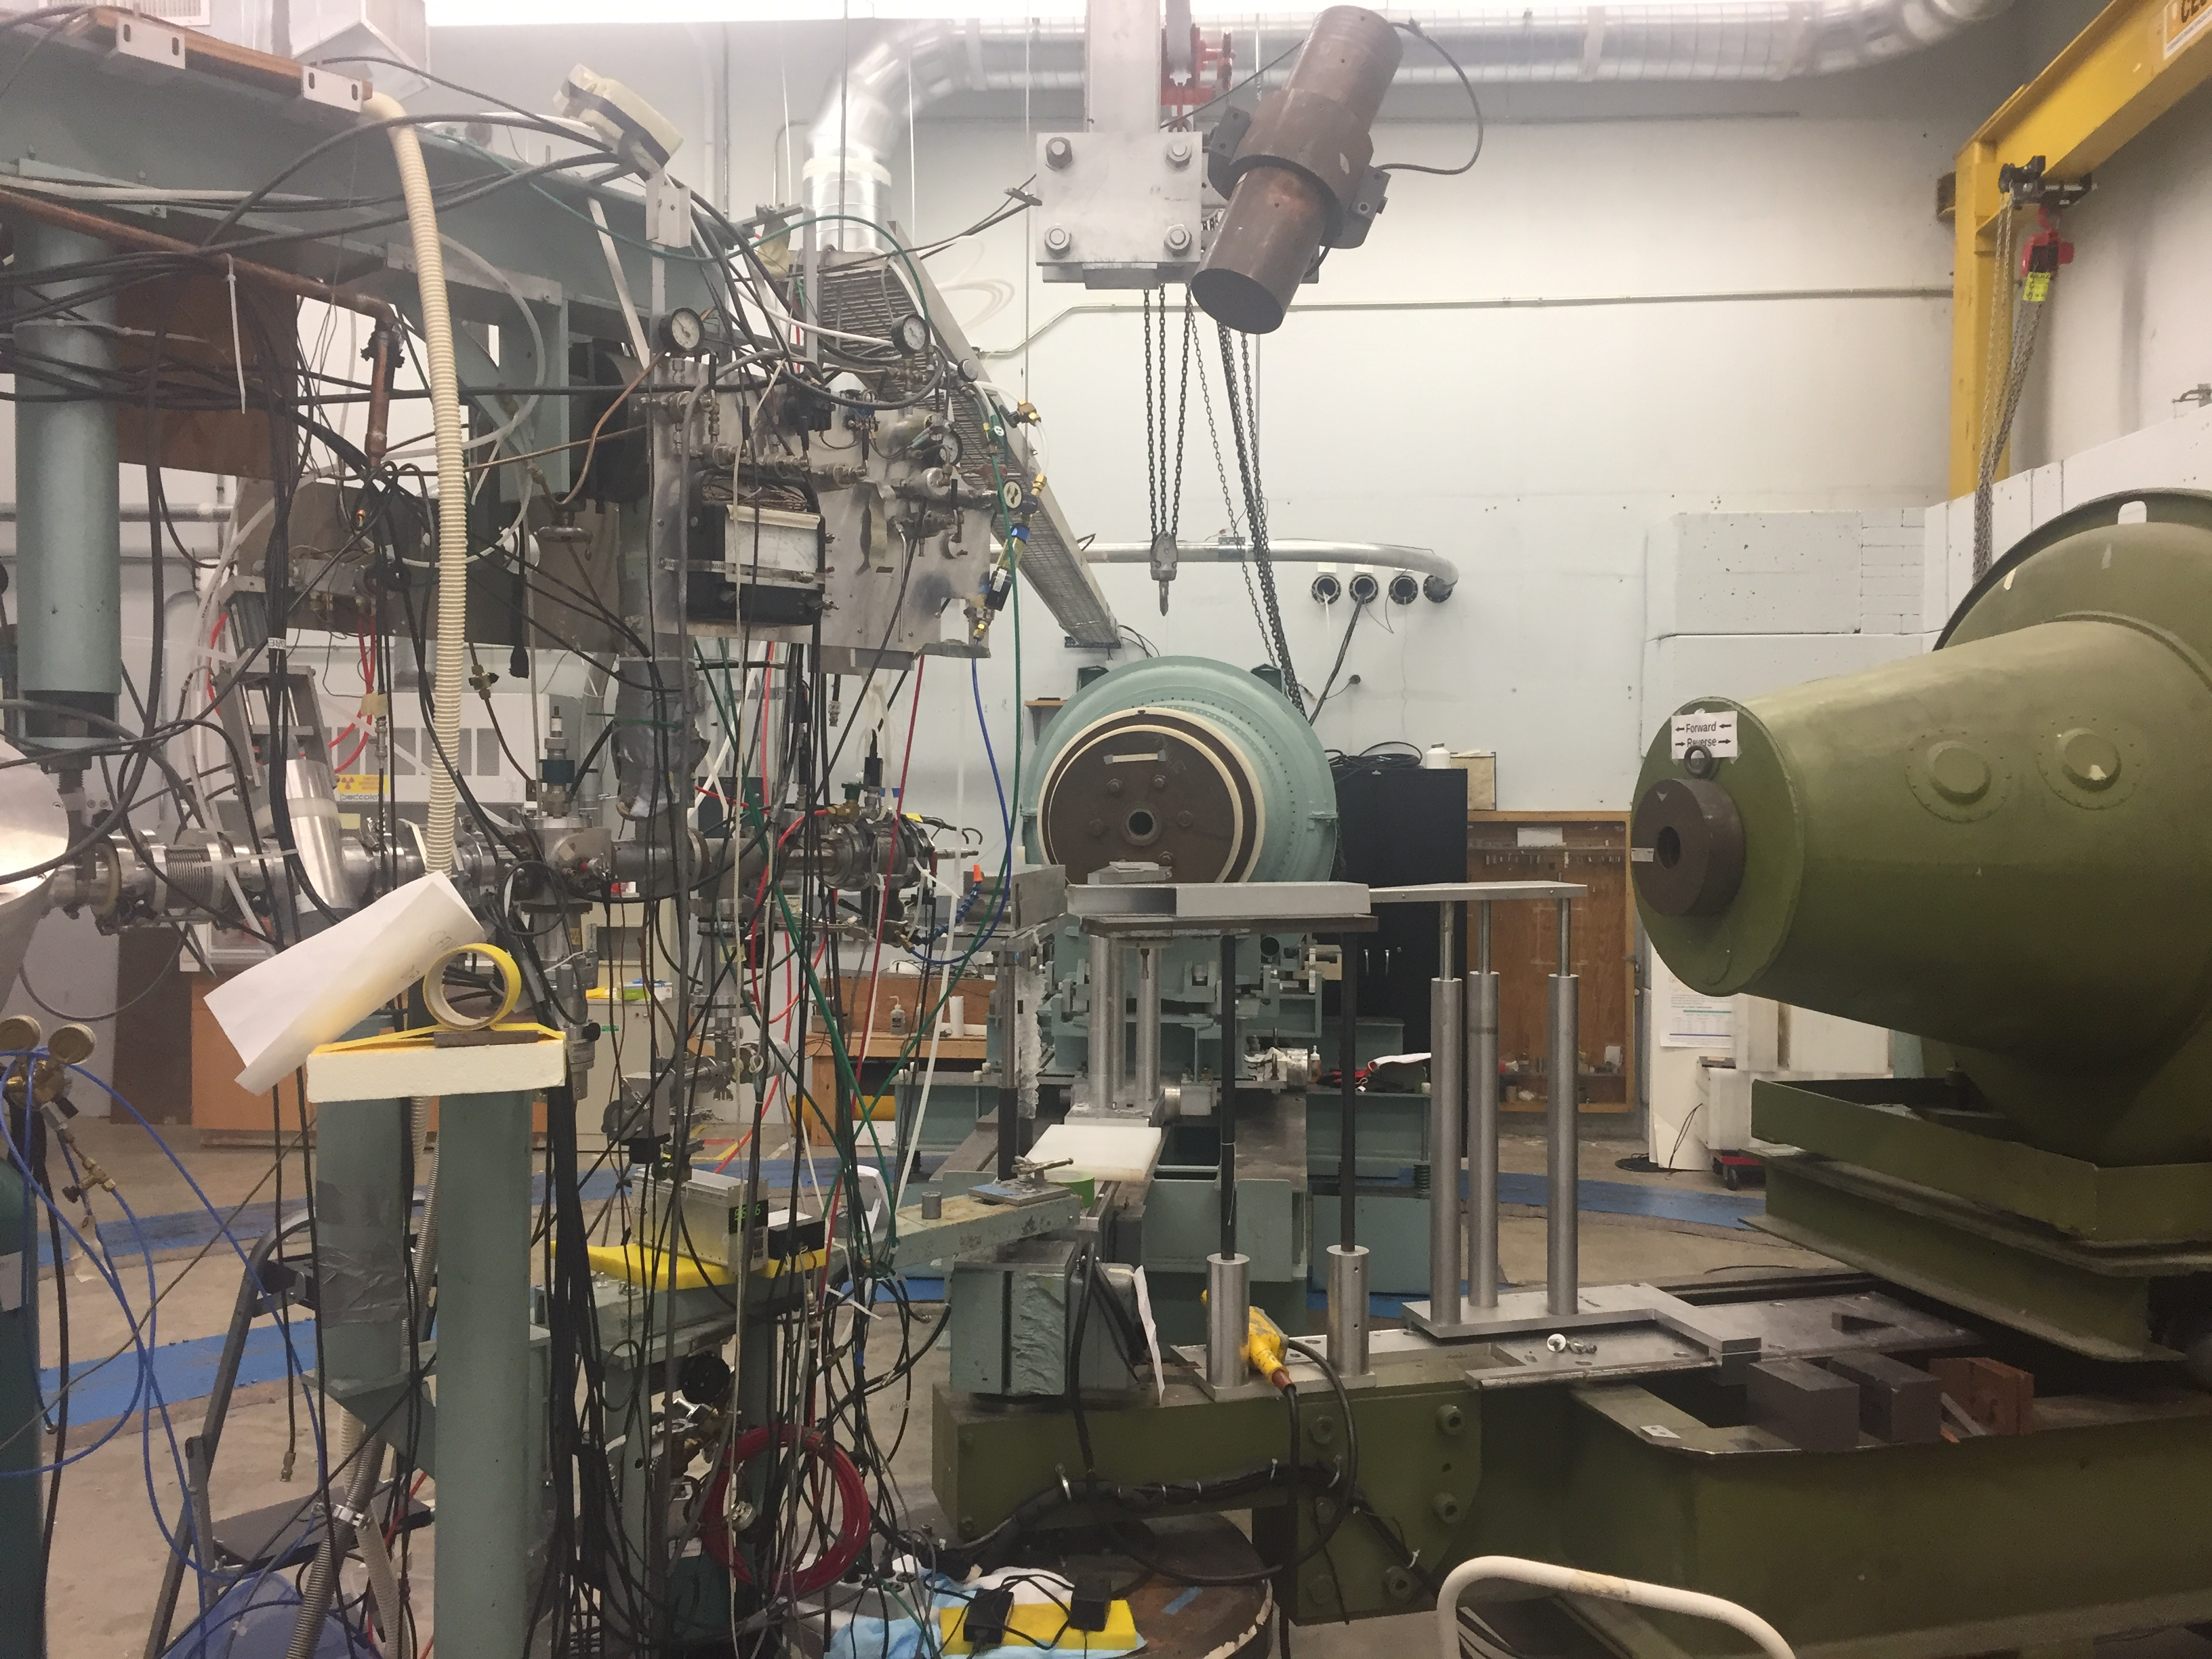
\includegraphics[width = 0.9\textwidth]{figures/TOFRoomPhoto.jpg}
    \caption[Image of the neutron TOF room at TUNL] 
    {
    Image of the neutron TOF room at TUNL. The deuteron beam pipe is visible on the left and
    terminates in a small deuteron gas target in the middle of the image, where neutrons are
    produced. The two detector arms are shown at center (6M) and right (4M). The ceiling
    monitor detector (CMON), which records beam flux, is visible at the top of the image.
    }
    \label{TOFRoomPhoto}
\end{figure}

\section{Data Acquisition}
Timing, pulse-shape discrimination, and pulse height information were
extracted by the analog signal processing logic laid out in Fig. \ref{ECSLogicDiagram}.
Raw signals from each neutron detector are processed by Mesytec MPD-4
pulse-shape-discrimination modules. The pulse tail length is converted to an
amplitude via a time-to-analog converter (TAC), providing neutron-gamma
discrimination. The pulse amplitude is measured by a separate
analog-to-digital converter (\gls{ADC}). Event times (labeled ``Gate'' from each MPD-4)
are passed as logic signals to a single time-to-digital converter (\gls{TDC}) so that
event times are recorded using a single clock. Pulse counts (``scalers'') are
collected at each step and the TDC, ADC, and data acquisition computer busy
signals are used to arrest the TDC when the system is already busy processing,
avoiding event pile-up.

\begin{sidewaysfigure}[tb]
    \centering
    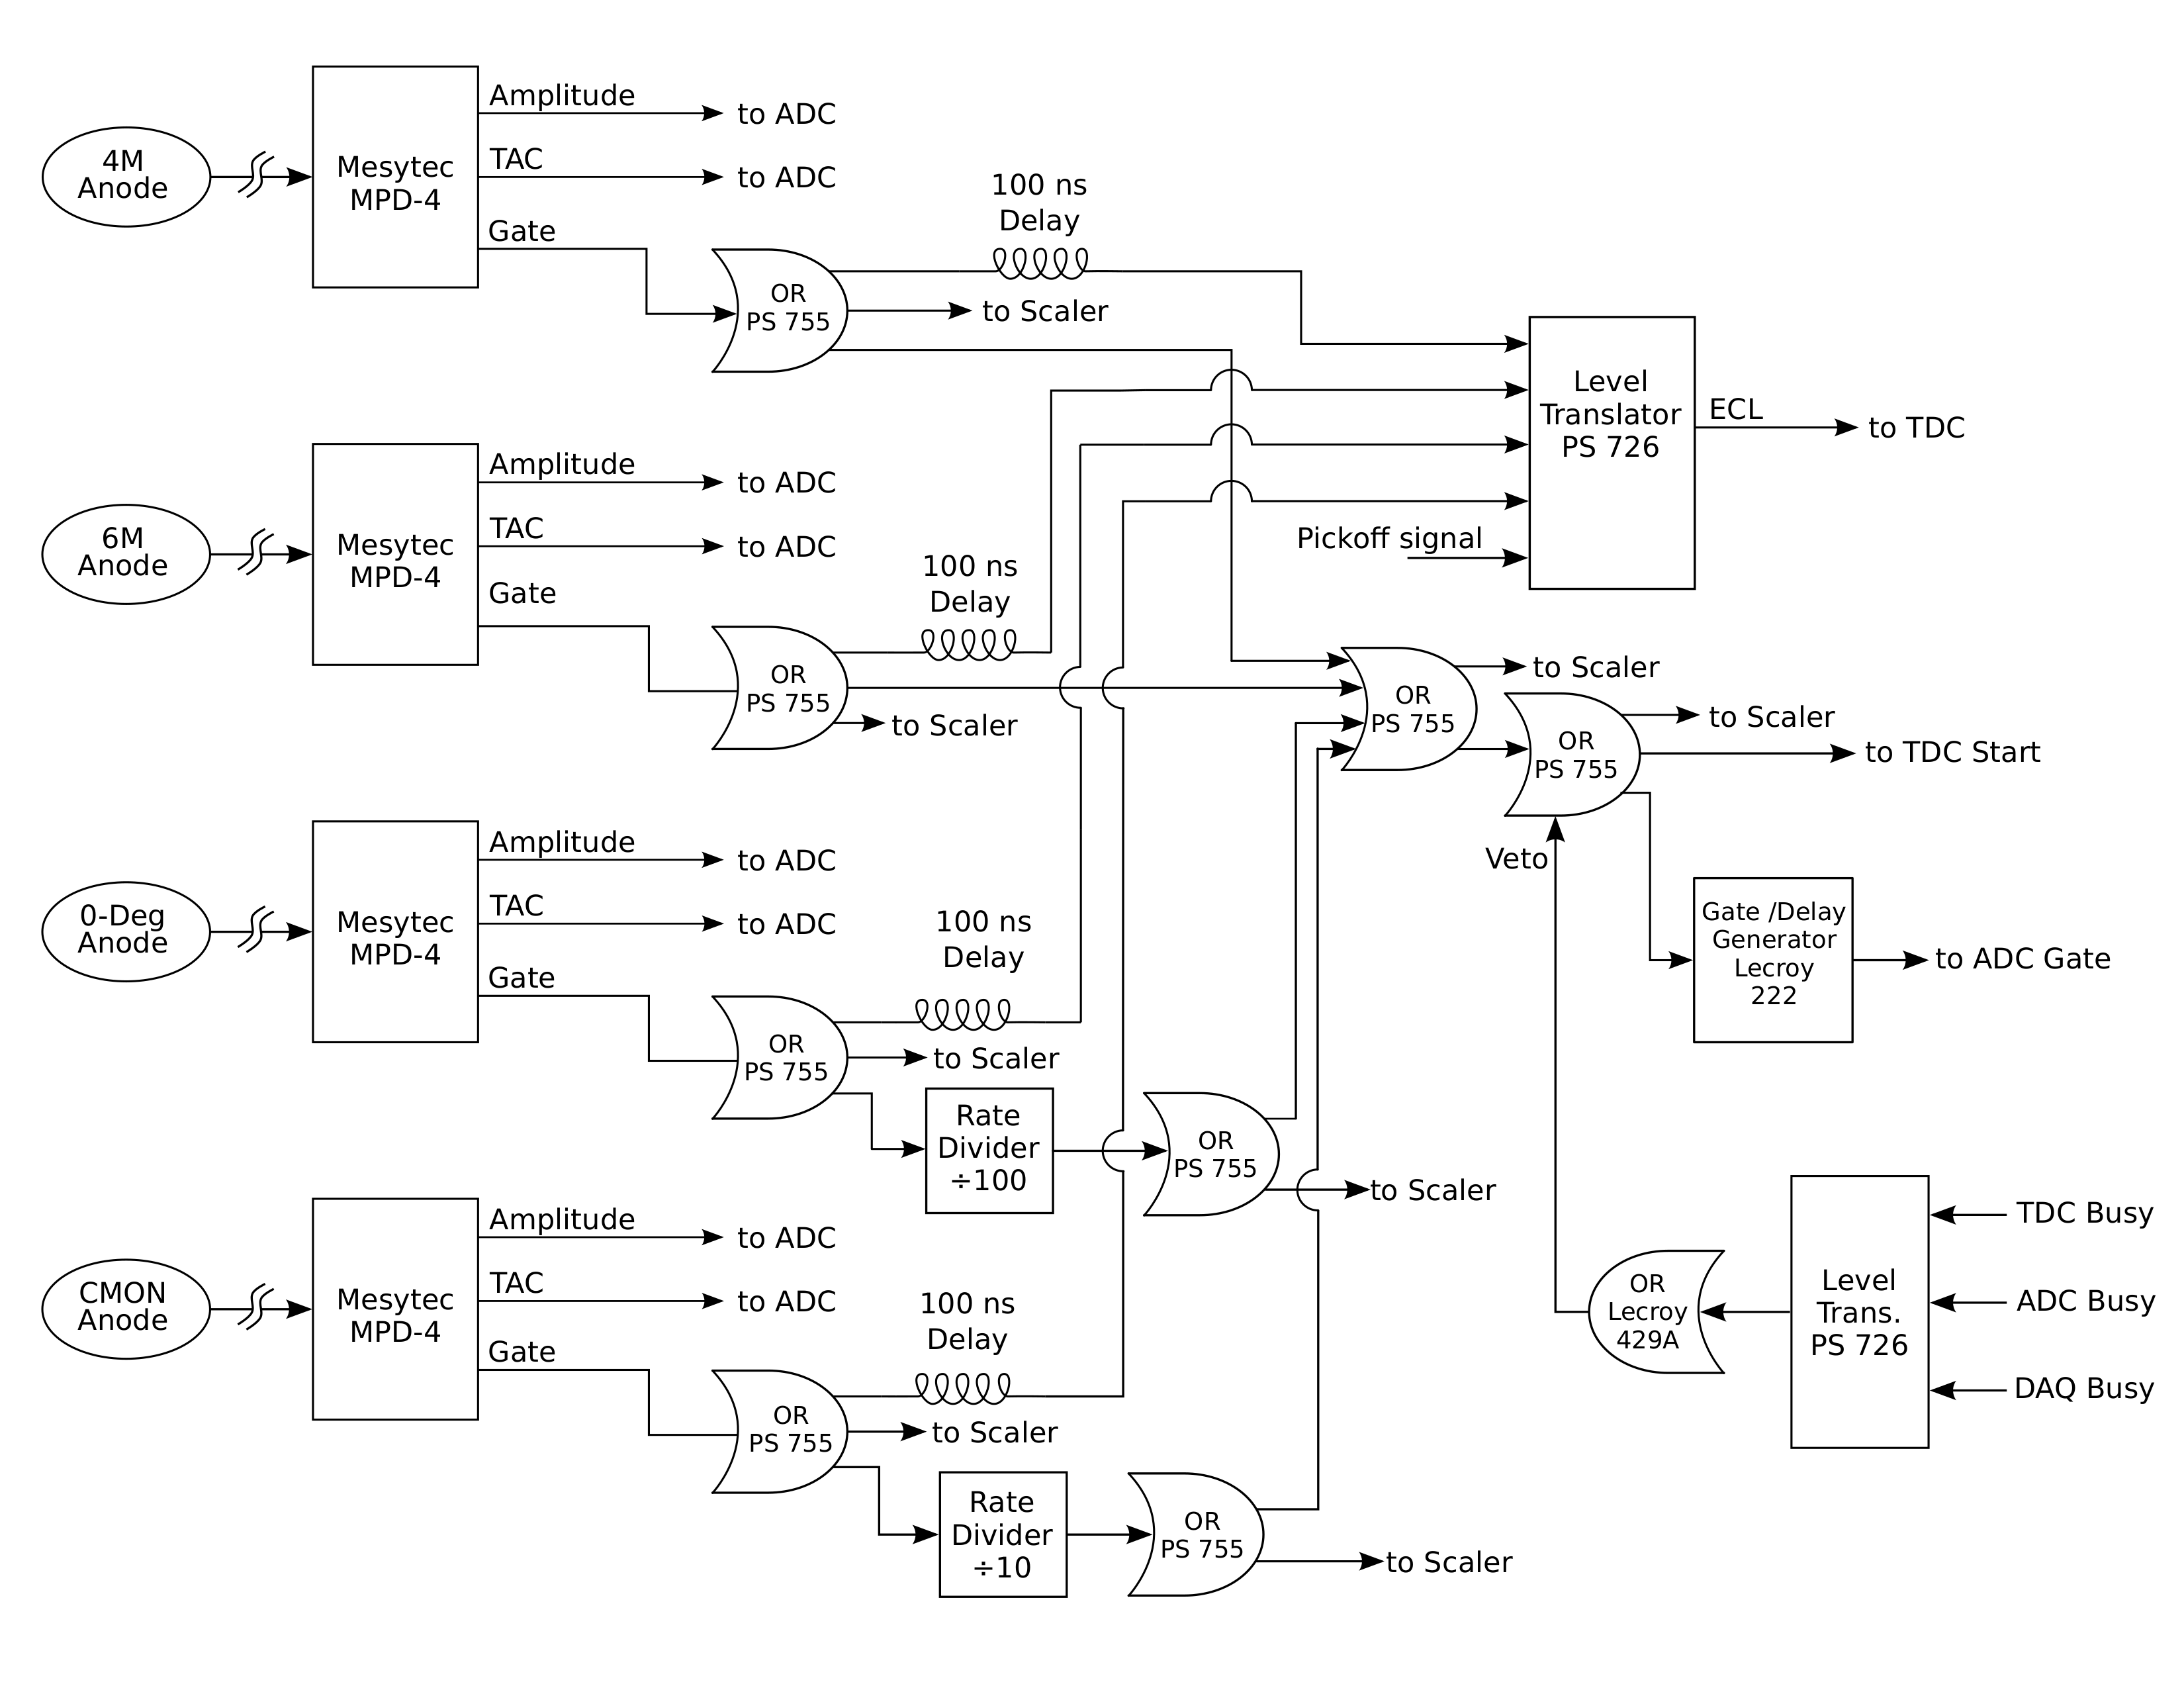
\includegraphics[width=0.9\textwidth]{figures/ECSLogic.png}
    \caption[Logic diagram for neutron \el\ data acquisition]
    {Logic diagram for neutron \el\ data acquisition at the TUNL time-of-flight
    room. Details are given in the text. Figure courtesy Ron Malone at TUNL.}
    \label{ECSLogicDiagram}
\end{sidewaysfigure}
